% Encoding:UTF-8
% Copyright 2014 MathFire
% Author: Rickjin (ZhihuiJin@gmail.com)
%
\chapter{认识Beta/Dirichlet分布}
\section{撒旦的游戏---认识Beta 分布}

统计学就是猜测上帝的游戏,当然我们不总是有机会猜测上帝,运气不好的时候就得揣度魔鬼的心思。
有一天你被魔鬼撒旦抓走了,撒旦说:“你们人类很聪明,而我是很仁慈的,
和你玩一个游戏,赢了就可以走,否则把灵魂出卖给我。
游戏的规则很简单,我有一个魔盒,上面有一个按钮,你每按一下按钮,
就均匀的输出一个[0,1]之间的随机数,我现在按10下,
我手上有10个数,你猜第7大的数是什么,偏离不超过0.01就算对。” 你应该怎么猜呢?

从数学的角度抽象一下,上面这个游戏描述如下
\begin{algorithm}[H]
\floatname{algorithm}{Game}
\caption{猜测第$k$ 大的数}
\begin{algorithmic}[1]
\STATE $X_1,X_2,\cdots,X_n {\stackrel{\mathrm{iid}}{\sim}} Uniform(0,1)$,
\STATE 把这$n$ 个随机变量排序后得到顺序统计量 $X_{(1)},X_{(2)},\cdots, X_{(n)}$,
\STATE 问 $X_{(k)}$ 的分布是什么
\end{algorithmic}
\end{algorithm}
对于不喜欢数学的同学而言,估计每个概率分布都是一个恶魔,那在概率统计学中,
均匀分布应该算得上是潘多拉魔盒,几乎所有重要的概率分布都可以从均匀分布$Uniform(0,1)$中生成出来。
\begin{figure}[htbp]
\centering
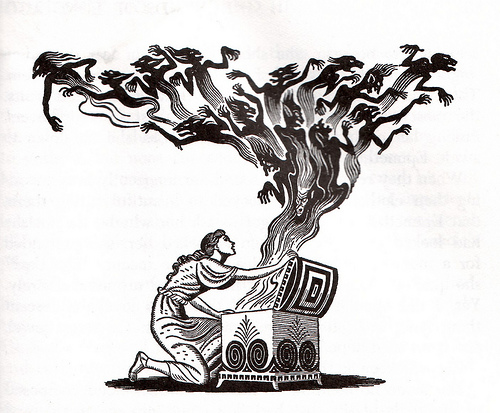
\includegraphics[width=0.6\textwidth]{lda/pandora.jpg}
\caption{潘多拉魔盒}
\end{figure}

对于上面的游戏而言 $n=10,k=7$, 如果我们能求出 $X_{(7)}$ 的分布的概率密度,那么用概率密度的极值点
去做猜测就是最好的策略。对于一般的情形,$X_{(k)}$ 的分布是什么呢?那我们尝试计算一下$X_{(k)}$ 落在
一个区间 $[x, x+\Delta x]$ 的概率,也就是求如下概率值
$$ P( x \le X_{(k)} \le x+\Delta x) = ? $$

把 [0,1] 区间分成三段 $[0,x), [x,x+\Delta x], (x+\Delta x,1]$,
我们先考虑简单的情形,假设$n$ 个数中只有一个落在了区间 $[x, x+\Delta x]$内,
则因为这个区间内的数$X_{(k)}$是第$k$大的,则$[0,x)$中应该有 $k-1$ 个数,$(x,1]$这个区间中应该有
$n-k$ 个数。不失一般性,我们先考虑如下一个符合上述要求的事件$E$
\begin{align*}
 E = \{ & X_1 \in [x, x+\Delta x],  \\
 & X_i \in [0,x)\quad (i=2,\cdots,k), \\
 & X_j \in (x+\Delta x,1] \quad (j=k+1,\cdots,n)\}
\end{align*}
\begin{figure}[htbp]
\centering
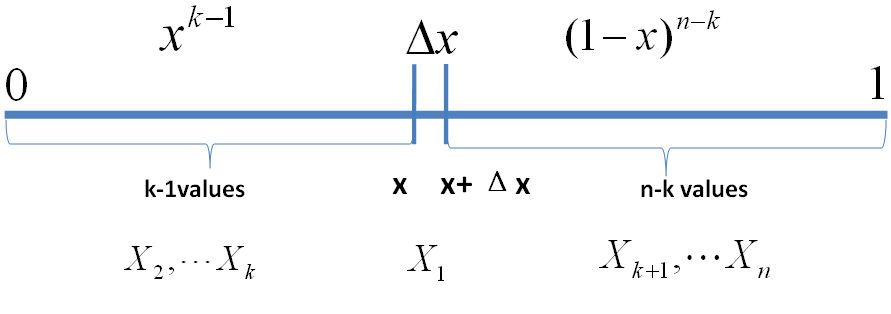
\includegraphics[width=0.8\textwidth]{lda/beta-game-1.png}
\caption{事件 $E$}
\end{figure}

则有
\begin{align*}
 P(E) & = \prod_{i=1}^nP(X_i) \\
 & = x^{k-1}(1-x-\Delta x)^{n-k}\Delta x \\
 & = x^{k-1}(1-x)^{n-k}\Delta x + o(\Delta x)
\end{align*}
$o(\Delta x)$表示$\Delta x $的高阶无穷小。
显然,由于不同的排列组合,即$n$个数中有一个落在 $[x, x+\Delta x]$区间的有$n$种取法,余下
$n-1$个数中有$k-1$个落在$[0,x)$的有$\binom{n-1}{k-1}$种组合,所以和事件$E$等价的事件一共有
$n\binom{n-1}{k-1}$个。

继续考虑稍微复杂一点情形,假设$n$ 个数中有两个数落在了区间 $[x, x+\Delta x]$,
\begin{align*}
E' = \{ & X_1,X_2\in [x, x+\Delta x], \\
& X_i \in [0,x) \quad (i=3,\cdots,k), \\
& X_j \in (x+\Delta x,1] \quad (j=k+1,\cdots,n)\}
\end{align*}
\begin{figure}[htbp]
\centering
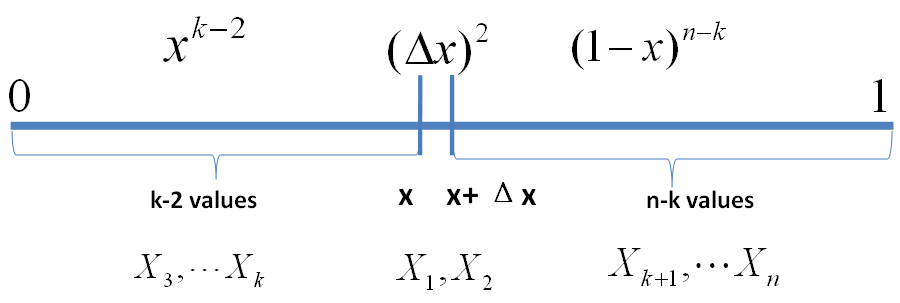
\includegraphics[width=0.8\textwidth]{lda/beta-game-2.png}
\caption{事件 $E'$}
\end{figure}

则有
$$ P(E') = x^{k-2}(1-x-\Delta x)^{n-k}(\Delta x)^2 = o(\Delta x)$$

从以上分析我们很容易看出,只要落在$[x, x+\Delta x]$内的数字超过一个,
则对应的事件的概率就是 $o(\Delta x)$。于是
\begin{align*}
& P( x \le X_{(k)} \le x+\Delta x) \\
& = n\binom{n-1}{k-1}P(E) + o(\Delta x) \\
& = n\binom{n-1}{k-1}x^{k-1}(1-x)^{n-k}\Delta x +  o(\Delta x)
\end{align*}
所以,可以得到$X_{(k)}$的概率密度函数为
\begin{align*}
f(x) & = \lim_{\Delta x \rightarrow 0} \frac{P( x \le X_{(k)} \le x+\Delta x)}{\Delta x} \\
& = n\binom{n-1}{k-1}x^{k-1}(1-x)^{n-k} \\
& = \frac{n!}{(k-1)!(n-k)!}x^{k-1}(1-x)^{n-k} \quad x \in [0,1]
\end{align*}
利用Gamma 函数,我们可以把 $f(x)$ 表达为
$$ f(x) = \frac{\Gamma(n+1)}{\Gamma(k)\Gamma(n-k+1)}x^{k-1}(1-x)^{n-k} $$
还记得神奇的 Gamma 函数可以把很多数学概念从整数集合延拓到实数集合吧。我们在上式中取
$\alpha=k, \beta=n-k+1$, 于是我们得到
\begin{equation}
f(x) = \frac{\Gamma(\alpha+\beta)}{\Gamma(\alpha)\Gamma(\beta)}x^{\alpha-1}(1-x)^{\beta-1}
\end{equation}
这个就是一般意义上的 Beta 分布!可以证明,在$\alpha,\beta$取非负实数的时候,这个概率密度函数也都是良定义的。

好,我们回到魔鬼的游戏,这$n=10,k=7$这个具体的实例中,我们按照如下密度分布的峰值去猜测才是最有把握的。
$$ f(x) = \frac{10!}{(6)!(3)!}x^{6}(1-x)^{3} \quad x \in [0,1] $$

然而即便如此,我们能做到一次猜中的概率也不高,很不幸,你第一次没有猜中,
魔鬼微笑着说:“我再仁慈一点,再给你一个机会,你按5下这个机器,
你就得到了5个[0,1]之间的随机数,然后我可以告诉你这5个数中的每一个,和我的第7大的数相比,
谁大谁小,然后你继续猜我手头的第7大的数是多少。”这时候我们应该怎么猜测呢?

\section{Beta-Binomial 共轭}
魔鬼的第二个题目,数学上形式化一下,就是
\begin{algorithm}[htb]
\floatname{algorithm}{Game}
\caption{继续猜测第$k$ 大的数}
\begin{algorithmic}[1]
\STATE $X_1,X_2,\cdots,X_n {\stackrel{\mathrm{iid}}{\sim}}Uniform(0,1)$,排序后对应的顺序统计量 $X_{(1)},X_{(2)},\cdots, X_{(n)}$,  我们要猜测 $p=X_{(k)}$;
\STATE $Y_1,Y_2,\cdots,Y_m {\stackrel{\mathrm{iid}}{\sim}}Uniform(0,1)$, $Y_i$中有$m_1$个比$p$小,$m_2$个比$p$大;
\STATE 问 $P(p|Y_1,Y_2,\cdots,Y_m)$ 的分布是什么。
\end{algorithmic}
\end{algorithm}

由于$p=X_{(k)}$在 $X_1,X_2,\cdots,X_n $中是第$k$大的,利用$Y_i$的信息,我们容易推理得到 $p=X_{(k)}$ 在
$X_1,X_2,\cdots,X_n,Y_1,Y_2,\cdots,Y_m {\stackrel{\mathrm{iid}}{\sim}} Uniform(0,1)$ 这$(m+n)$个独立随机变量中是第 $k+m_1$大的,
于是按照上一个小节的推理,此时$p=X_{(k)}$ 的概率密度函数是 $Beta(p|k+m_1,n-k+1+m_2)$。
按照贝叶斯推理的逻辑,我们把以上过程整理如下:
\begin{enumerate}
\item $p=X_{(k)}$是我们要猜测的参数,我们推导出 $p$ 的分布为 $f(p) = Beta(p|k,n-k+1)$,称为 $p$ 的先验分布;
\item 数据$Y_i$中有$m_1$个比$p$小,$m_2$个比$p$大,$Y_i$相当于是做了$m$次贝努利实验,所以$m_1$ 服从二项分布 $B(m,p)$;
\item 在给定了来自数据提供的$(m_1,m_2)$的知识后,$p$ 的后验分布变为 $f(p|m_1,m_2)=Beta(p|k+m_1,n-k+1+m_2)$
\end{enumerate}
\begin{figure}[htbp]
\centering

\includegraphics[width=0.2\textwidth]{lda/coin-toss.jpg}
\caption{贝努利实验}
\end{figure}
我们知道贝叶斯参数估计的基本过程是
\begin{center}
 \bf{先验分布 + 数据的知识  = 后验分布}
\end{center}
以上贝叶斯分析过程的简单直观的表述就是
$$ Beta(p|k,n-k+1) + BinomCount(m_1,m_2) = Beta(p|k+m_1,n-k+1+m_2) $$
其中 $(m_1,m_2)$ 对应的是二项分布$B(m_1+m_2,p)$的计数。
更一般的,对于非负实数$\alpha,\beta$,我们有如下关系
\begin{equation}
 Beta(p|\alpha,\beta) + BinomCount(m_1,m_2) = Beta(p|\alpha+m_1,\beta+m_2)
\end{equation}
这个式子实际上描述的就是 {\bf Beta-Binomial 共轭},此处共轭的意思就是,
数据符合二项分布的时候,参数的先验分布和后验分布都能保持Beta 分布的形式,
这种形式不变的好处是,我们能够在先验分布中赋予参数很明确的物理意义,
这个物理意义可以延续到后验分布中进行解释,
同时从先验变换到后验过程中从数据中补充的知识也容易有物理解释。

而我们从以上过程可以看到,
Beta 分布中的参数$\alpha,\beta$都可以理解为物理计数,这两个参数经常被称为伪计数(pseudo-count)。
基于以上逻辑,我们也可以把$Beta(p|\alpha,\beta)$写成下式来理解
\begin{equation}
\label{uniform-beta}
Beta(p|1,1) + BinomCount(\alpha-1,\beta-1) = Beta(p|\alpha,\beta)
\end{equation}
其中 $Beta(p|1,1)$ 恰好就是均匀分布$Uniform(0,1)$。

对于\eqref{uniform-beta}式,我们其实也可以纯粹从贝叶斯的角度来进行推导和理解。
假设有一个不均匀的硬币抛出正面的概率为$p$,抛$m$次后出现正面和反面的次数分别是$m_1,m_2$,
那么按传统的频率学派观点,$p$的估计值应该为 $\hat{p}=\frac{m_1}{m}$。而从贝叶斯学派的观点来看,
开始对硬币不均匀性一无所知,所以应该假设$p\sim Uniform(0,1)$, 于是有了二项分布的计数$(m_1,m_2)$
之后,按照贝叶斯公式如下计算$p$ 的后验分布
\begin{align*}
P(p|m_1,m_2)  & = \frac{P(p)\cdot P(m_1,m_2|p)}{P(m_1,m_2)} \\
& = \frac{1\cdot P(m_1,m_2|p)}{\int_0^1 P(m_1,m_2|t)dt} \\
& = \frac{\binom{m}{m_1}p^{m_1}(1-p)^{m_2}}{\int_0^1 \binom{m}{m_1}t^{m_1}(1-t)^{m_2}dt} \\
& = \frac{p^{m_1}(1-p)^{m_2}}{\int_0^1 t^{m_1}(1-t)^{m_2}dt}
\end{align*}
计算得到的后验分布正好是 $Beta(p|m_1+1,m_2+1)$。

\begin{figure}[htbp]
\centering
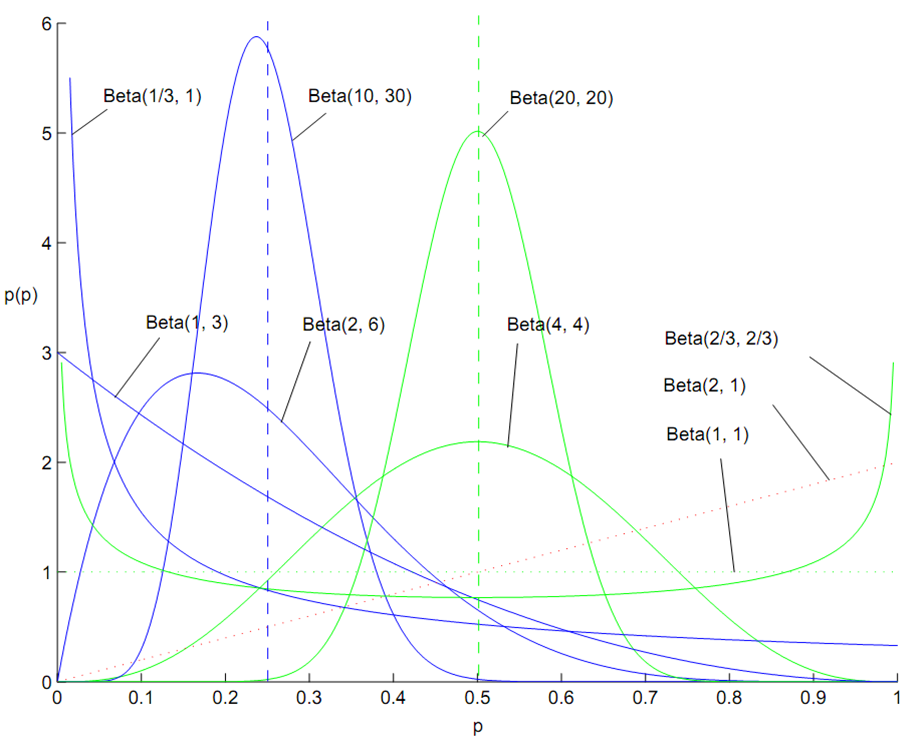
\includegraphics[width=0.8\textwidth]{lda/beta-distribution.png}
\caption{百变星君Beta分布}
\end{figure}
Beta 分布的概率密度我们把它画成图,会发现它是个百变星君,它可以是凹的、凸的、单调上升的、单调下降的;
可以是曲线也可以是直线,而均匀分布也是特殊的Beta分布,读者请参看一个网站上的
\href{http://www.aiaccess.net/English/Glossaries/GlosMod/e_gm_beta_distri.htm}{Beta 分布 Demo},
通过调节参数$\alpha,\beta$ 可以观察 Beta 分布的各种形态。。由于Beta 分布能够拟合如此之多的形状,
因此它在统计数据拟合和贝叶斯分析中被广泛使用。

在上一个小节中,我们从二项分布推导Gamma 分布的时候,使用了如下的等式
\begin{equation}
\label{binomial-beta2}
P(C \le k) = \frac{n!}{k!(n-k-1)!} \int_p^1 t^k(1-t)^{n-k-1} dt,  \quad  C\sim B(n,p)
\end{equation}
现在大家可以看到,左边是二项分布的概率累积,右边实际上是$Beta(t|k+1,n-k)$ 分布的概率积分。
这个式子在上一小节中并没有给出证明,下面我们利用和魔鬼的游戏类似的概率物理过程进行证明。

我们可以如下构造二项分布,取随机变量 $X_1, X_2, \cdots, X_n {\stackrel{\mathrm{iid}}{\sim}}Uniform(0,1)$,
一个成功的贝努利实验就是 $X_i<p$,否则表示失败,于是成功的概率为$p$。
$C$用于计数成功的次数,于是$C\sim B(n,p)$。
\begin{figure}[H]
\centering
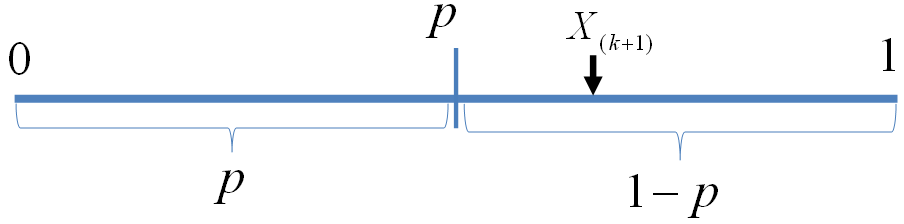
\includegraphics[width=0.8\textwidth]{lda/beta-binomial.png}
\caption{贝努利实验最多成功$k$次}
\end{figure}
显然我们有如下式子成立
$$ P(C \le k) = P(X_{(k+1)} > p)$$
此处$X_{(k+1)}$是顺序统计量,为第$k+1$大的数。
等式左边表示贝努利实验成功次数最多$k$次,右边表示第 $k+1$ 大的数必然对应于失败的贝努利实验,
从而失败次数最少是$n-k$次,所以左右两边是等价的。
由于$X_{(k+1)} \sim Beta(t|k+1, n-k)$, 于是
\begin{align*}
P(C \le k) & = P(X_{(k+1)} > p) \\
&= \int_p^1 Beta(t|k+1, n-k)dt \\
&= \frac{n!}{k!(n-k-1)!} \int_p^1 t^k(1-t)^{n-k-1} dt
\end{align*}

最后我们再回到魔鬼的游戏,如果你按出的5个随机数字中,魔鬼告诉你有2个小于它手中第7大的数,
那么你应该按照如下概率分布的峰值做猜测是最好的
$$ Beta(x|9,7) = \frac{15!}{(8)!(6)!}x^{8}(1-x)^{6} \quad x \in [0,1] $$

很幸运的,你这次猜中了,魔鬼开始甩赖了:这个游戏对你来说太简单了,
我要加大点难度,我们重新来一次,我按魔盒20下生成20个随机数,
你同时给我猜第7大和第13大的数是什么,这时候应该如何猜测呢?

\section{Dirichlet-Multinomial 共轭}
对于魔鬼变本加厉的新的游戏规则,数学形式化如下:
\begin{algorithm}[htb]
\floatname{algorithm}{Game}
\caption{猜测第$k_1$ 大和第$k_1+k_2$大的数}
\begin{algorithmic}[1]
\STATE $X_1,X_2,\cdots,X_n {\stackrel{\mathrm{iid}}{\sim}}Uniform(0,1)$,
\STATE 排序后对应的顺序统计量 $X_{(1)},X_{(2)},\cdots, X_{(n)}$,
\STATE 问 $(X_{(k_1)}, X_{(k_1+k_2)})$的联合分布是什么;
\end{algorithmic}
\end{algorithm}

完全类似于第一个游戏的推导过程,我们可以进行如下的概率计算
(为了数学公式的简洁对称,我们取$x_3$满足$x_1+x_2+x_3 = 1$,但只有$x_1,x_2$是变量)
\begin{figure}[htbp]
\centering
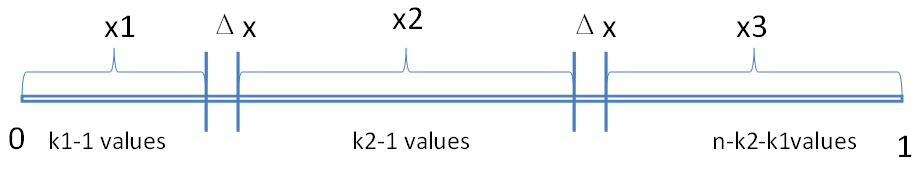
\includegraphics[width=0.8\textwidth]{lda/dirichlet-game.png}
\caption{$(X_{(k_1)}, X_{(k_1+k_2)})$的联合分布推导}
\end{figure}
\begin{align*}
& P\Bigl(X_{(k_1)}\in(x_1,x_1+\Delta x),X_{(k_1+k_2)}\in(x_1+x_2,x_1+x_2+\Delta x)\Bigr) \\
& = n(n-1)\binom{n-2}{k_1-1,k_2-1}x_1^{k_1-1}x_2^{k_2-1}x_3^{n-k_1-k_2}(\Delta x)^2 \\
& = \frac{n!}{(k_1-1)!(k_2-1)!(n-k_1-k_2)!}x_1^{k_1-1}x_2^{k_2-1}x_3^{n-k_1-k_2}(\Delta x)^2
\end{align*}
于是我们得到 $(X_{(k_1)}, X_{(k_1+k_2)})$的联合分布是
\begin{align*}
f(x_1,x_2,x_3) & = \frac{n!}{(k_1-1)!(k_2-1)!(n-k_1-k_2)!}x_1^{k_1-1}x_2^{k_2-1}x_3^{n-k_1-k_2} \\
& = \frac{\Gamma(n+1)}{\Gamma(k_1)\Gamma(k_2)\Gamma(n-k_1-k_2+1)}x_1^{k_1-1}x_2^{k_2-1}x_3^{n-k_1-k_2}
\end{align*}
熟悉 Dirichlet的同学一眼就可以看出,上面这个分布其实就是3维形式的 Dirichlet 分布
$Dir(x_1,x_2,x_3|k_1,k_2,n-k_1-k_2+1)$。
令 $\alpha_1=k_1,\alpha_2=k_2,\alpha_3=n-k_1-k_2+1$,于是分布密度可以写为
\begin{equation}
\displaystyle f(x_1,x_2,x_3) = \frac{\Gamma(\alpha_1 + \alpha_2 + \alpha_3)}
{\Gamma(\alpha_1)\Gamma(\alpha_2)\Gamma(\alpha_3)}x_1^{\alpha_1-1}x_2^{\alpha_2-1}x_3^{\alpha_3-1}
\end{equation}

这个就是一般形式的3维 Dirichlet 分布,即便 $\vec{\alpha}=(\alpha_1,\alpha_2, \alpha_3)$ 延拓
到非负实数集合,以上概率分布也是良定义的。

从形式上我们也能看出,Dirichlet 分布是Beta 分布在高维度上的推广,他和Beta 分布一样也是一个百变星君,
密度函数可以展现出多种形态。
\begin{figure}[htbp]
\centering
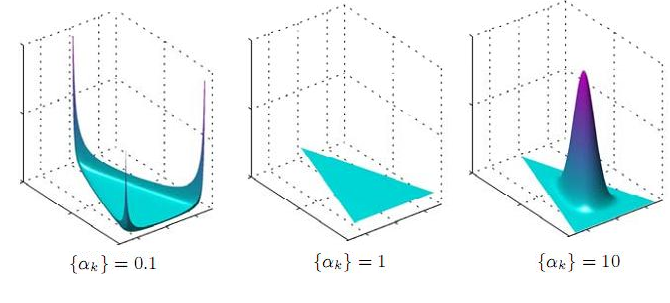
\includegraphics[width=0.8\textwidth]{lda/dirichlet-distribution.png}
\caption{不同 $\alpha$ 下的Dirichlet 分布}
\end{figure}


类似于魔鬼的游戏2,我们也可以调整一下游戏3,从魔盒中生成$m$个随机数
$Y_1,Y_2,\cdots,Y_m {\stackrel{\mathrm{iid}}{\sim}}Uniform(0,1)$
并让魔鬼告诉我们$Y_i$和$(X_{(k_1)}, X_{(k_1+k_2)})$相比谁大谁小。于是有如下游戏4
\begin{algorithm}[htb]
\floatname{algorithm}{Game}
\caption{继续猜测第$k_1$ 大和第$k_1+k_2$大的数}
\begin{algorithmic}[1]
\STATE $X_1,X_2,\cdots,X_n {\stackrel{\mathrm{iid}}{\sim}}Uniform(0,1)$,排序后对应的顺序统计量 $X_{(1)},X_{(2)},\cdots, X_{(n)}$
\STATE 令$p_1=X_{(k_1)}, p_2=X_{(k_1+k_2)},p_3 = 1-p_1-p_2$(加上$p_3$是为了数学表达简洁对称),
我们要猜测 $\vec{p}=(p_1,p_2,p_3)$;
\STATE $Y_1,Y_2,\cdots,Y_m {\stackrel{\mathrm{iid}}{\sim}}Uniform(0,1)$, $Y_i$中落到
$[0,p_1),[p_1,p_2),[p_2,1]$ 三个区间的个数分别为 $m_1,m_2,m_3$,$m=m_1+m_2+m3$;
\STATE 问后验分布 $P(\vec{p}|Y_1,Y_2,\cdots,Y_m)$ 的分布是什么。
\end{algorithmic}
\end{algorithm}

为了方便,我们记
$$ \vec{m}=(m_1,m_2,m_3),\quad \vec{k}=(k_1,k_2,n-k_1-k_2+1) $$
由游戏中的信息,我们可以推理得到 $p_1, p_2$在
$X_1,X_2,\cdots,X_n,$ $Y_1,Y_2,\cdots,Y_m$
${\stackrel{\mathrm{iid}}{\sim}} Uniform(0,1)$
这 $m+n$个数中分别成为了第 $k_1+m_1, k_2+m_2$大的数,于是后验分布 $P(\vec{p}|Y_1,Y_2,\cdots,Y_m)$
应该是 $Dir(\vec{p}|k_1+m_1,k_1+m_2,n-k_1-k_2+1+m_3)$,即
$Dir(\vec{p}|\vec{k}+\vec{m})$。
按照贝叶斯推理的逻辑,我们同样可以把以上过程整理如下:
\begin{enumerate}
\item 我们要猜测参数 $\vec{p}=(p_1,p_2,p_3)$,其先验分布为$Dir(\vec{p}|\vec{k})$;
\item 数据$Y_i$落到$[0,p_1), [p_1,p_2),[p_2,1]$三个区间的个数分别为 $m_1,m_2,m_3$,所以
$\vec{m}=(m_1,m_2,m_3)$ 服从多项分布$Mult(\vec{m}|\vec{p})$
\item 在给定了来自数据提供的知识$\vec{m}$后,$\vec{p}$ 的后验分布变为 $Dir(\vec{p}|\vec{k}+\vec{m})$
\end{enumerate}
以上贝叶斯分析过程的简单直观的表述就是
$$ Dir(\vec{p}|\vec{k}) + MultCount(\vec{m}) = Dir(\vec{p}|\vec{k}+\vec{m}) $$
令 $\vec{\alpha}=\vec{k}$,把$\vec{\alpha}$
从整数集合延拓到实数集合,更一般的可以证明有如下关系
\begin{equation}
 Dir(\vec{p}|\vec{\alpha}) + MultCount(\vec{m})
 = Dir(\vec{p}|\vec{\alpha}+\vec{m})
\end{equation}
以上式子实际上描述的就是 {\bf Dirichlet-Multinomial 共轭},而我们从以上过程可以看到,
Dirichlet 分布中的参数$\vec{\alpha}$都可以理解为物理计数。
类似于 Beta 分布,我们也可以把 $Dir(\vec{p}|\vec{\alpha})$作如下分解
$$ Dir(\vec{p}|\vec{1}) + MultCount(\vec{m}-\vec{1})
= Dir(\vec{p}|\vec{\alpha}) $$
此处$\vec{1}=(1,1,\cdots,1)$。自然,上式我们也可以类似地用纯粹贝叶斯的观点进行推导和解释。

以上的游戏我们还可以往更高的维度上继续推,譬如猜测 $X_{(1)},X_{(2)},\cdots, X_{(n)}$ 中的
4、5、...等更多个数,于是就得到更高纬度的 Dirichlet 分布和 Dirichlet-Multinomial 共轭。
一般形式的 Dirichlet 分布定义如下
\begin{equation}
\displaystyle Dir(\vec{p}|\vec{\alpha}) =
\displaystyle \frac{\Gamma(\sum_{k=1}^K\alpha_k)}
{\prod_{k=1}^K\Gamma(\alpha_k)} \prod_{k=1}^K p_k^{\alpha_k-1}
\end{equation}
对于给定的 $\vec{p}$和 $N$,多项分布定义为
\begin{equation}
\displaystyle  Mult(\vec{n} |\vec{p},N) = \binom{N}{\vec{n}}\prod_{k=1}^K p_k^{n_k}
\end{equation}
而 $Mult(\vec{n} |\vec{p},N)$ 和 $Dir(\vec{p}|\vec{\alpha})$
这两个分布是共轭关系。

Beta-Binomail 共轭和 Dirichlet-Multinomail 共轭都可以用纯粹数学的方式进行证明,我们在这两个小节中通过一个游戏
来解释这两个共轭关系,主要是想说明这个共轭关系是可以对应到很具体的概率物理过程的。

\section{Beta/Dirichlet 分布的一个性质}

如果 $p\sim Beta(t|\alpha,\beta)$, 则
\begin{align*}
E(p) & = \int_0^1 t*Beta(t|\alpha,\beta)dt \\
& =  \int_0^1 t* \frac{\Gamma(\alpha+\beta)}{\Gamma(\alpha)\Gamma(\beta)} t^{\alpha-1}(1-t)^{\beta-1}dt \\
& = \frac{\Gamma(\alpha+\beta)}{\Gamma(\alpha)\Gamma(\beta)}  \int_0^1 t^{\alpha}(1-t)^{\beta-1}dt
\end{align*}
上式右边的积分对应到概率分布 $Beta(t|\alpha+1,\beta)$,对于这个分布,我们有
$$
\int_0^1 \frac{\Gamma(\alpha+\beta+1)}{\Gamma(\alpha+1)\Gamma(\beta)} t^{\alpha}(1-t)^{\beta-1}dt = 1
$$
把上式带入$E(p)$的计算式,得到
\begin{align}
E(p) & = \frac{\Gamma(\alpha+\beta)}{\Gamma(\alpha)\Gamma(\beta)}
\cdot \frac{\Gamma(\alpha+1)\Gamma(\beta)}{\Gamma(\alpha+\beta+1)} \notag \\
& = \frac{\Gamma(\alpha+\beta)}{\Gamma(\alpha+\beta+1)}\frac{\Gamma(\alpha+1)}{\Gamma(\alpha)} \notag \\
& = \frac{\alpha}{\alpha+\beta}
\label{beta-mean}
\end{align}
这说明,对于Beta 分布的随机变量,其均值可以用$\frac{\alpha}{\alpha+\beta}$来估计。
Dirichlet 分布也有类似的结论,
如果$\vec{p} \sim Dir(\vec{t}|\vec{\alpha})$,同样可以证明
\begin{equation}
 E(\vec{p}) = \Bigl(\frac{\alpha_1}{\sum_{i=1}^K\alpha_i},\frac{\alpha_2}{\sum_{i=1}^K\alpha_i},\cdots, \frac{\alpha_K}{\sum_{i=1}^K\alpha_i} \Bigr)
 \label{dir-mean}
\end{equation}
以上两个结论很重要,因为我们在后面的 LDA 数学推导中需要使用这个结论。


